\begin{figure}[tbh]
\centering
\subfigure[Exponential Growing \textsc{CTEvent} Size: $y=2^x$]{
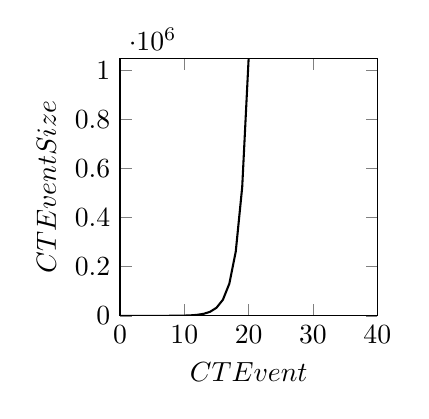
\begin{tikzpicture}
  \begin{axis}[ 
  width=0.4\linewidth,
      height=0.4\textwidth,
    xlabel=$CTEvent$,
    ylabel={$CTEvent Size$},
    xmin=0.00, xmax=40,
	ymin=0, ymax=1048576
  ] 
    \addplot [
    line width=0.75pt]
    coordinates {
    		(0.00, 1.00)
		(1.00, 2.00)
		(2.00, 4.00)
		(3.00, 8.00)
		(4.00, 16.00)
		(5.00, 32.00)
		(6.00, 64.00)
		(7.00, 128.00)
		(8.00, 256.00)
		(9.00, 512.00)
		(10.00, 1024.00)
		(11.00, 2048.00)
		(12.00, 4096.00)
		(13.00, 8192.00)
		(14.00, 16384.00)
		(15.00, 32768.00)
		(16.00, 65536.00)
		(17.00, 131072.00)
		(18.00, 262144.00)
		(19.00, 524288.00)
		(20.00, 1048576.00)
		};	
		
	\end{axis}
\normalsize

\end{tikzpicture}
}
\subfigure[Step Growing Size with K1=100 and K2=1000 after 9 \textsc{CTEvents}]{
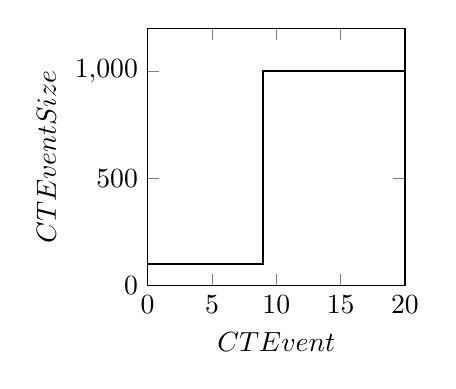
\begin{tikzpicture}
  \begin{axis}[ 
  width=0.4\linewidth,
      height=0.4\textwidth,
    xlabel=$CTEvent$,
    ylabel={$CTEvent Size$},
    xmin=0.00, xmax=20,
	ymin=0, ymax=1200
  ] 
    \addplot [
    line width=0.75pt]
    coordinates {
    		(0.00, 100.00)
		(1.00, 100.00)
		(2.00, 100.00)
		(3.00, 100.00)
		(4.00, 100.00)
		(5.00, 100.00)
		(6.00, 100.00)
		(7.00, 100.00)
		(8.00, 100.00)
		(9.00, 100.00)
		(9.00, 1000.00)
		(10.00, 1000.00)
		(11.00, 1000.00)
		(12.00, 1000.00)
		(13.00, 1000.00)
		(14.00, 1000.00)
		(15.00, 1000.00)
		(16.00, 1000.00)
		(17.00, 1000.00)
		(18.00, 1000.00)
		(19.00, 1000.00)
		(20.00, 1000.00)
		};	
		
	\end{axis}
\normalsize

\end{tikzpicture}
}
\caption[Example of FlowRateProfiler Triple Distribution]{The \textsc{FlowRateProfiler} is able to calculate \textsc{CTEvent} size according to a function which relates the number of triple to the number of \textsc{CTEvent}.}
\label{fig:frp-examples}
\end{figure}
